\subsection{Initial temperature for melting}

When looking at the simulation in Ovito, we found that the melting point seems to be around an initial temperature of 600 K \cite{ovito}. We added the displacement of the atoms to the movie-file, so we could color code the displacement of the atom, to make it easier to see the melting. Figure \ref{fig:solid_100K} shows the supercell when it is clearly solid and Figure \ref{fig:solid_600K}, Figure \ref{fig:almost_melted_600K} and Figure \ref{fig:melted_600K} shows the development from the ordered initial FCC structure to the melted state. The red color represent a displacement of 6 Å or more, the blue a displacement near 0 Å and the green is a medium displacement, around 3 Å. 

\begin{multicols}{2}

\begin{figure}[H]
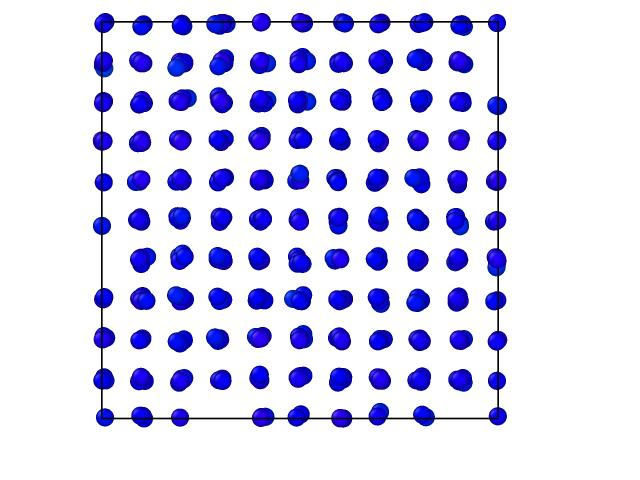
\includegraphics[width=\linewidth]{../figures/solid_100}\caption{This is a snap shot of the supercell of argon with an initial temperature of 100 K. The structure is clearly solid, with some lattice vibration due to nonzero temperature. The picture is form Ovito \cite{ovito}.}\label{fig:solid_100K}
\end{figure}

\begin{figure}[H]
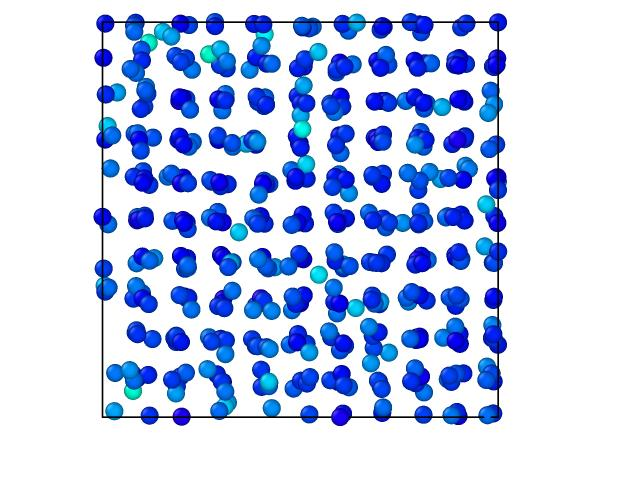
\includegraphics[width=\linewidth]{../figures/solid_600}\caption{This is a snap shot of the supercell of argon with an initial temperature of 600 K. The structure looks solid in the beginning. The picture is form Ovito \cite{ovito}.}\label{fig:solid_600K}
\end{figure}

\begin{figure}[H]
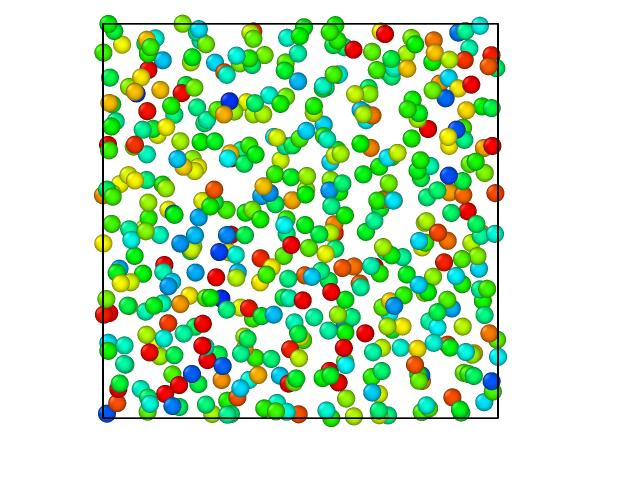
\includegraphics[width=\linewidth]{../figures/middle_melted_600}\caption{This is a snap shot of the supercell of argon with an initial temperature of 600 K. The structure is not solid, the displacement has increased. The picture is form Ovito \cite{ovito}.}\label{fig:almost_melted_600K}
\end{figure}

\begin{figure}[H]
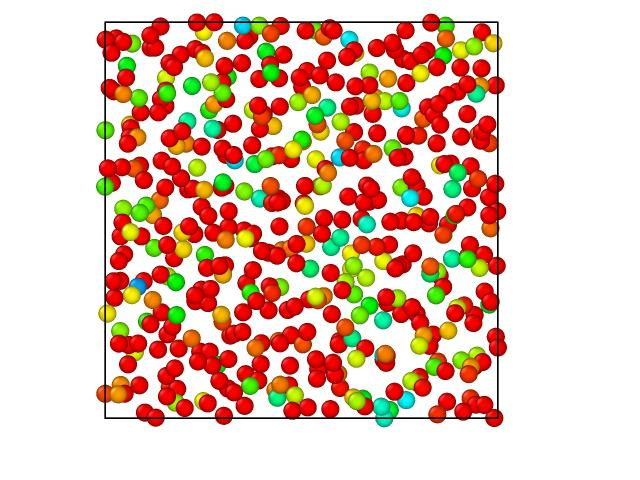
\includegraphics[width=\linewidth]{../figures/melted_600}\caption{This is a snap shot of the supercell of argon with an initial temperature of 600 K. The structure has melted almost all atoms are displaced by 6 Å or more. The picture is form Ovito \cite{ovito}.}\label{fig:melted_600K}
\end{figure}

\end{multicols}

\subsection{Real melting temperature}

The system starts in a very ordered state, so the potential energy is very low. The atoms were given random velocities from the Maxwell-Boltzmann distribution, so in the first time step the atoms have moved away from this high symmetric low potential state and the potential energy increases very much. Because the total energy has to be conserved, the kinetic energy start at a maximum and decreases a lot to compensate. The drop in kinetic energy gives a drop in temperature because of the relation between them (see Equation \ref{eq:equipartition}.). Equation \ref{eq:equipartition} is only accurate in thermal equilibrium, considering that, the initial temperatures are not that relevant. Figure \ref{fig:temperature} shows the development of the temperature with time. The temperature is approximately half the initial temperature in equilibrium. 

\begin{figure}[H]
\center
\includegraphics[width=0.8\linewidth]{../figures/temp_development}\caption{This is a  plot of the ratio between the initial temperature and the temperature calculated from the kinetic energy (see Equation \ref{eq:equipartition}) to show how it decreases to an equilibrium which is approximately half the initial temperature.}\label{fig:temperature}
\end{figure}

As a consequence of the temperature development, we chose to use the average of temperature form the kinetic energy at the last 10 \% of the time ($6\cdot 10^{-12}$ s) to find the temperature at equilibrium.

\subsection{Energy}

Figure \ref{fig:energy} shows the kinetic, the potential and the total energy of the system initially and how it reaches an equilibrium, where it fluctuate with a small amplitude. The figure shows how the potential starts in a minimum and the kinetic in a maximum. The total energy seems to be well converged. 

\begin{figure}[H]
\center
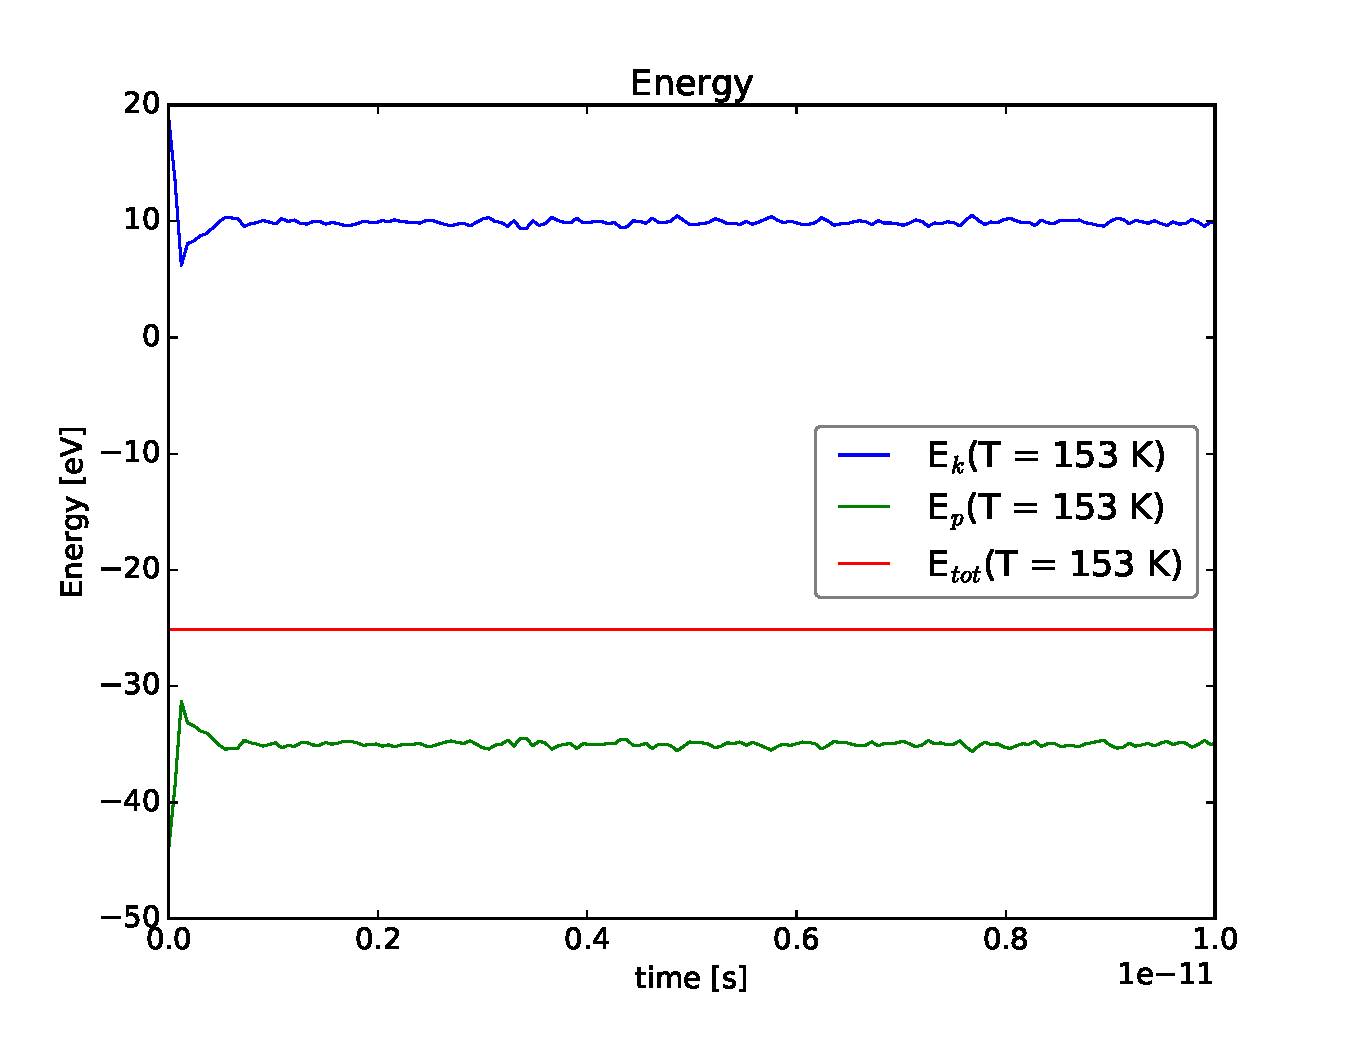
\includegraphics[width=0.8\linewidth]{../figures/energy}\caption{This is a plot of the energy at initial temperature 300 K and equilibrium temperature 153 K. The plot shows how the potential energy starts in a minimum and the kinetic in a maximum, and how the total energy is well conserved even though both the kinetic and potential fluctuates.}\label{fig:energy}
\end{figure}

\subsection{Diffusion constant}

Figure \ref{fig:below_melting} is a plot of the mean square displacement against temperature. According to the Einstein relation it should be a linear plot with slope $6D$, where $D$ is the diffusion constant. We did a linear regression on the data and extracted the diffusion constant for different temperatures. The temperatures in the legend are the equilibrium temperatures.

%\begin{multicols}{2}

\begin{figure}[H]
\center
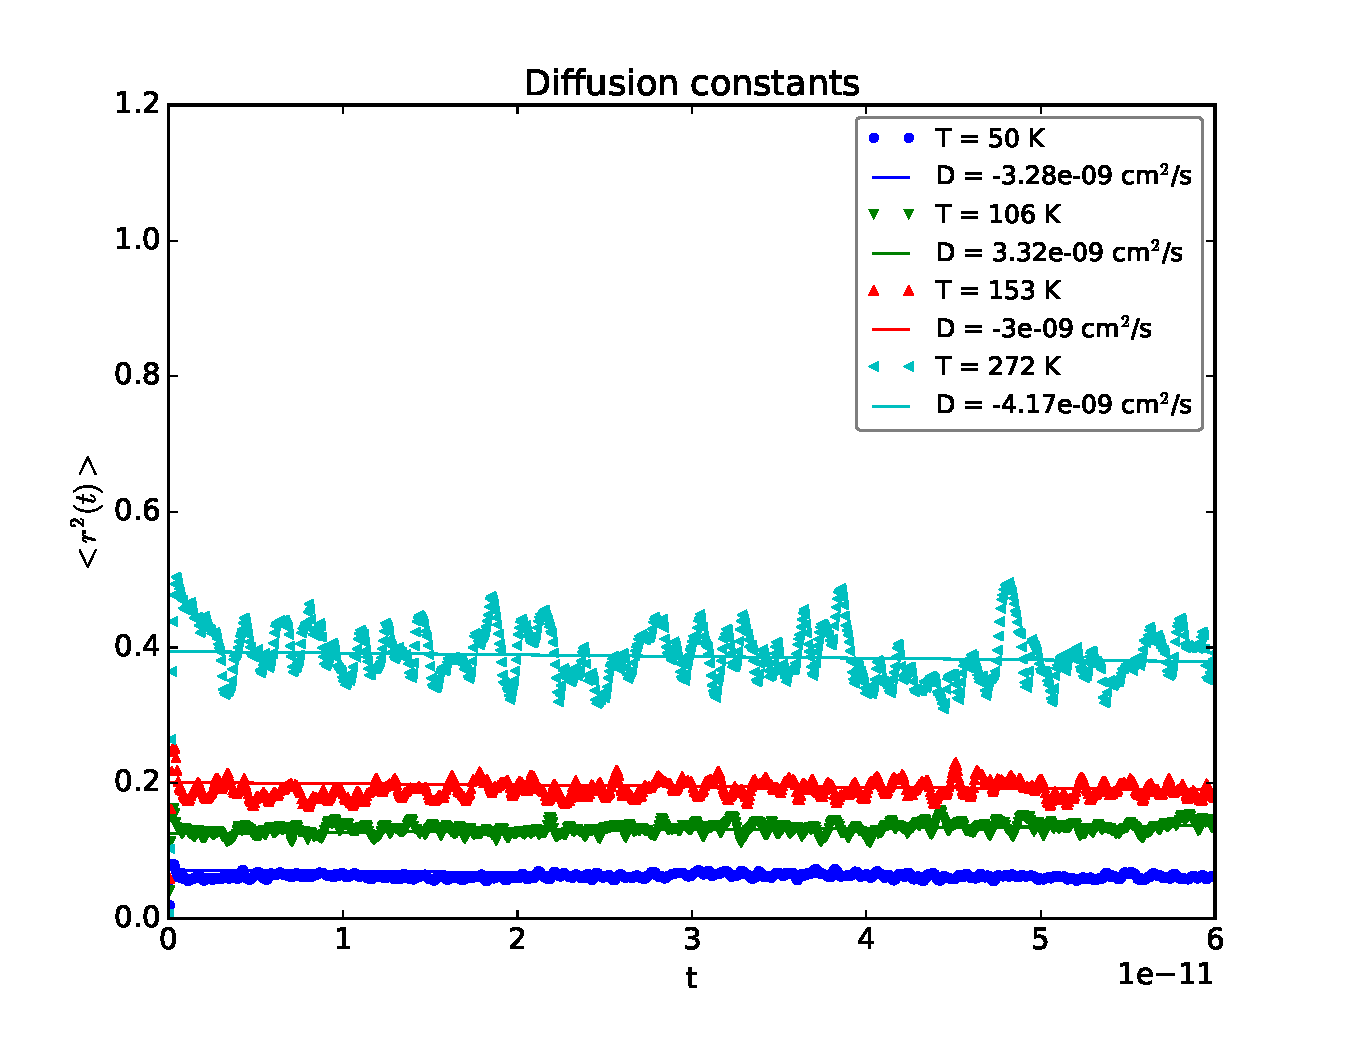
\includegraphics[width=0.8\linewidth]{../figures/below_melting}\caption{This is a plot of Einstein relation (see Equation \ref{eq:equipartition}), the diffusion constant is extraced from the slope of the linear regression. The temperatures are below the melting point.}\label{fig:below_melting}
\end{figure}

Figure \ref{fig:above_melting} is a plot of the mean square displacement against temperatures above the melting temperature. Because most of the data series has a kink and Equation \ref{eq:Einstein} shows a linear relation, we chose to use the last half of the data to do the linear regression and extract the diffusion constant form that. We assumed that the equilibrium had to be reached and that it was reached after $3\cdot 10^{-11}$ seconds.

\begin{figure}[H]
\center
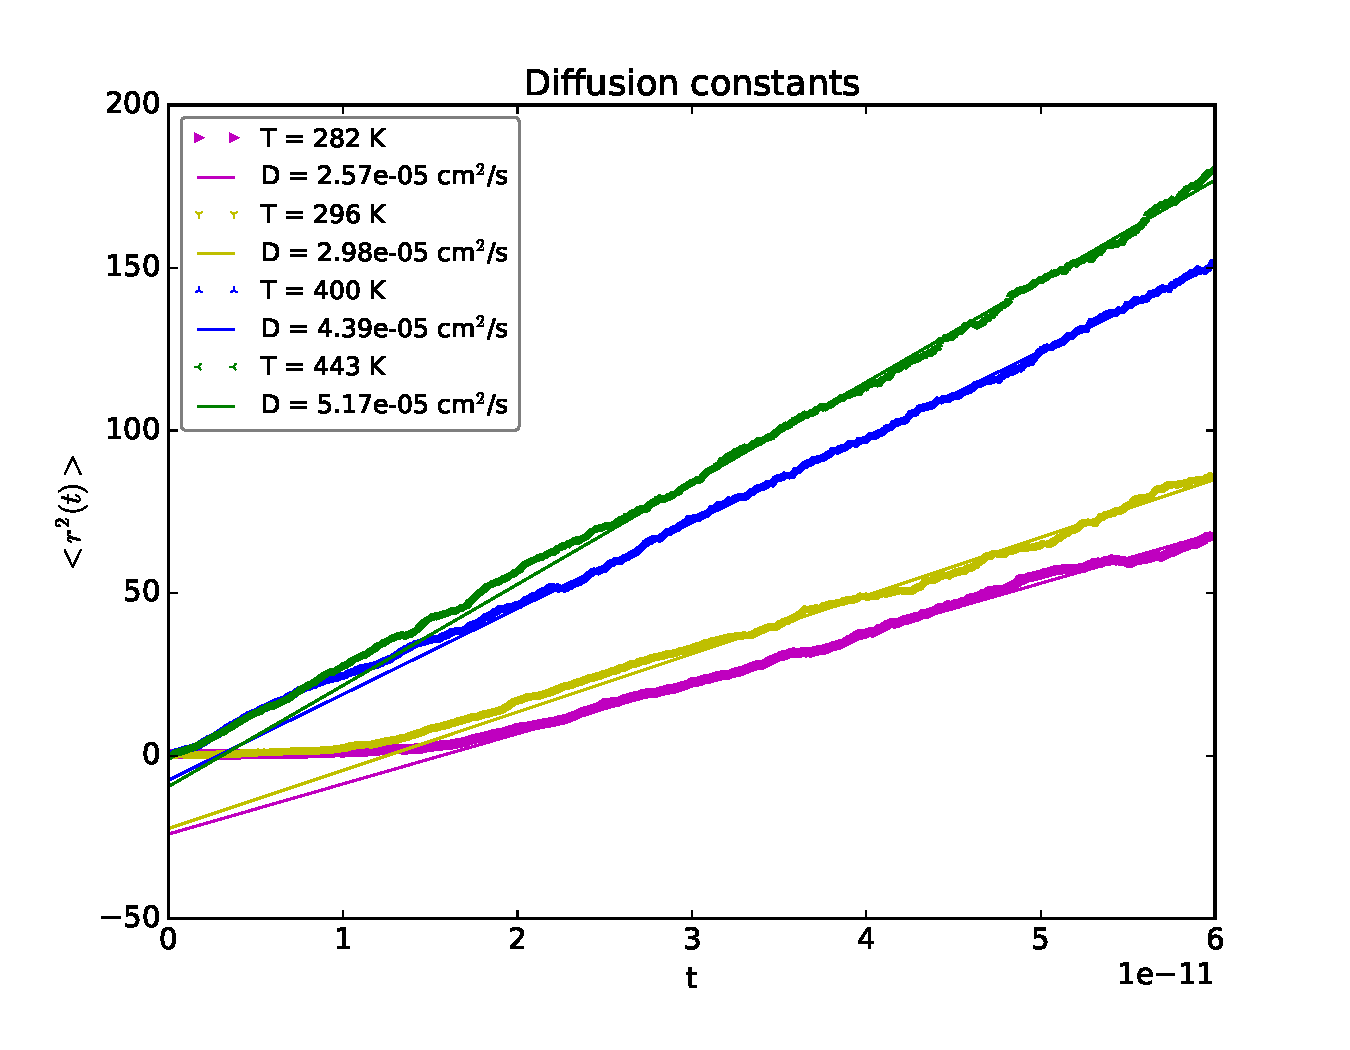
\includegraphics[width=0.8\linewidth]{../figures/above_melting}\caption{This is a plot of Einstein relation (see Equation \ref{eq:Einstein}), the diffusion constant is extraced from the slope of the linear regression. The temperatures are above the melting point.}\label{fig:above_melting}
\end{figure}

%\end{multicols}

The diffusion constants from Figure \ref{fig:below_melting} and Figure \ref{fig:above_melting} were plotted against temperature in Figure \ref{fig:diffusion_temp}. The diffusivity makes a jump at around 300 K, implying that the melting temperature is around 300 K. The values before the jump is around $10^{-9}$ cm$^2$/s (see Figure \ref{fig:below_melting}) which match the values for solids and the values after the melting matches the values for diffusion in liquids. This might suggest that it is a transition from solid to liquid.

\begin{figure}[H]
\center
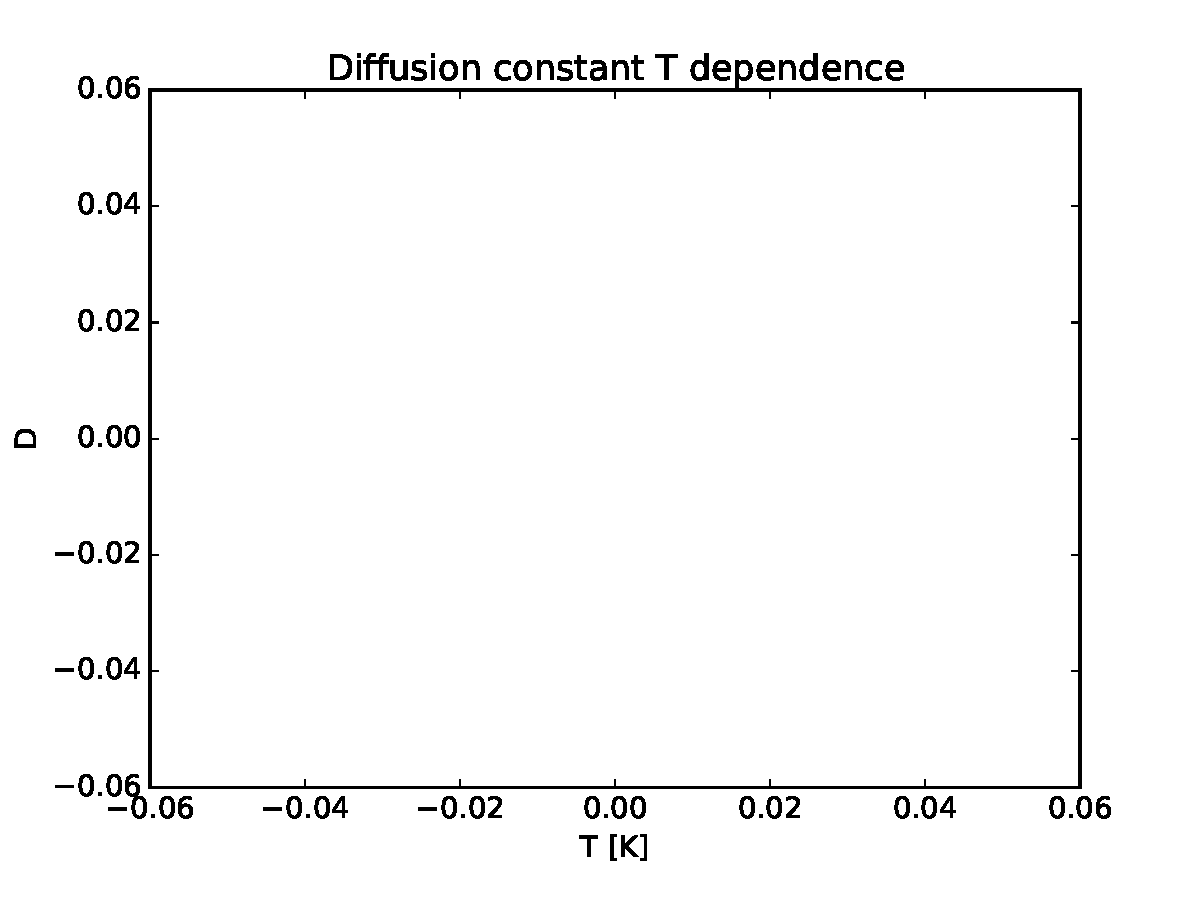
\includegraphics[width=0.8\linewidth]{../figures/diffusion_temp}\caption{This is a plot of the diffusion constant with respect to temperature. The values are taken from the slope of the linear regression of the mean squared distance versus time because of Einsteins relation (see Equation \ref{eq:Einstein}). The plot shows how the diffusion constant increases drastically after the melting point around 300 K.}\label{fig:diffusion_temp}
\end{figure}


The highest temperature with the relatively low diffusion constant is at $T = 272$ K and the highest with the high diffusion constants are at $T = 282$ K. That implies that the melting temperature is in the interval 272 K to 282 K. The system behave strangely around the melting temperature though, as Figure \ref{fig:near_Tc} shows, so it was difficult to set a specific melting point.

\begin{figure}[H]
\center
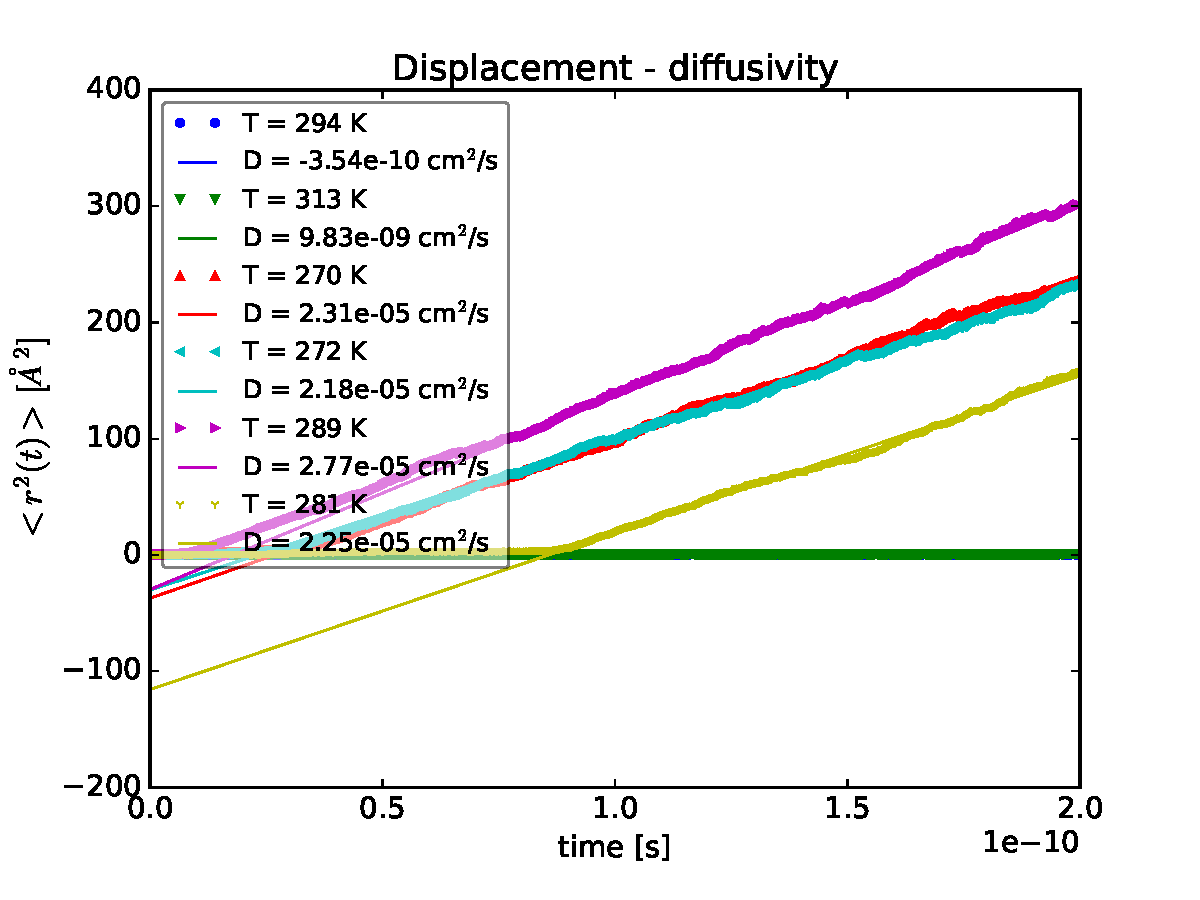
\includegraphics[width=0.8\linewidth]{../figures/nearTc}\caption{This shows the mean square displacement near the melting temperature showing some weird result, that the highest temperatures have the smallest slopes and then also the lowest diffusion constants. These runs were done for a longer time because of the temperature development around the melting point (see Figure \ref{fig:temp_development_nearTc}).}\label{fig:near_Tc}
\end{figure}

The experimental melting temperature of argon is 84 K at 1 atm pressure, and thus a lot smaller than our result. The reason might be that the pressure is not 1 atm. Since we do not calculate the pressure, it is difficult to check our result with phase diagrams plotted from experiments. Phase transitions are dependent on both temperature and pressure, so our result might be accurate for another pressure.

\subsection{Equilibrium temperature}

Figure \ref{fig:temp_development_all} shows the temperature development with different initial temperatures. The temperature development shows that the system with temperatures around melting point do not reach a proper equilibrium in the same timespan as the others. There is a shift after some time, making the results strange. Figure \ref{fig:temp_development_nearTc} shows the temperature development of system with initial temperatures that result in temperatures around the melting point. The program was run for a longer time span to get better diffusion constants (see Figure \ref{fig:near_Tc}) because of the shift in temperature.

\begin{figure}[H]
\center
\includegraphics[width=0.8\linewidth]{../figures/temp_development_all}\caption{This is a plot of the temperature development of systems with different initial temperatures. The system with initial temperatures that end up around the melting temperatures (600 K and 700 K) makes a shift after a while.}\label{fig:temp_development_all}
\end{figure}

\begin{figure}[H]
\center
\includegraphics[width=0.8\linewidth]{../figures/temp_development_nearTc_long}\caption{This is a plot of the temperature development of systems with different initial temperatures around the melting temperature. This might explain the strange numbers around the melting temperature.}\label{fig:temp_development_nearTc}
\end{figure}
